\documentclass[]{article}
\usepackage{lmodern}
\usepackage{amssymb,amsmath}
\usepackage{ifxetex,ifluatex}
\usepackage{fixltx2e} % provides \textsubscript
\ifnum 0\ifxetex 1\fi\ifluatex 1\fi=0 % if pdftex
  \usepackage[T1]{fontenc}
  \usepackage[utf8]{inputenc}
\else % if luatex or xelatex
  \ifxetex
    \usepackage{mathspec}
  \else
    \usepackage{fontspec}
  \fi
  \defaultfontfeatures{Ligatures=TeX,Scale=MatchLowercase}
\fi
% use upquote if available, for straight quotes in verbatim environments
\IfFileExists{upquote.sty}{\usepackage{upquote}}{}
% use microtype if available
\IfFileExists{microtype.sty}{%
\usepackage{microtype}
\UseMicrotypeSet[protrusion]{basicmath} % disable protrusion for tt fonts
}{}
\usepackage[margin=1in]{geometry}
\usepackage{hyperref}
\hypersetup{unicode=true,
            pdftitle={Reproducible Research: Peer Assessment 1},
            pdfauthor={James Francisco},
            pdfborder={0 0 0},
            breaklinks=true}
\urlstyle{same}  % don't use monospace font for urls
\usepackage{color}
\usepackage{fancyvrb}
\newcommand{\VerbBar}{|}
\newcommand{\VERB}{\Verb[commandchars=\\\{\}]}
\DefineVerbatimEnvironment{Highlighting}{Verbatim}{commandchars=\\\{\}}
% Add ',fontsize=\small' for more characters per line
\usepackage{framed}
\definecolor{shadecolor}{RGB}{248,248,248}
\newenvironment{Shaded}{\begin{snugshade}}{\end{snugshade}}
\newcommand{\KeywordTok}[1]{\textcolor[rgb]{0.13,0.29,0.53}{\textbf{#1}}}
\newcommand{\DataTypeTok}[1]{\textcolor[rgb]{0.13,0.29,0.53}{#1}}
\newcommand{\DecValTok}[1]{\textcolor[rgb]{0.00,0.00,0.81}{#1}}
\newcommand{\BaseNTok}[1]{\textcolor[rgb]{0.00,0.00,0.81}{#1}}
\newcommand{\FloatTok}[1]{\textcolor[rgb]{0.00,0.00,0.81}{#1}}
\newcommand{\ConstantTok}[1]{\textcolor[rgb]{0.00,0.00,0.00}{#1}}
\newcommand{\CharTok}[1]{\textcolor[rgb]{0.31,0.60,0.02}{#1}}
\newcommand{\SpecialCharTok}[1]{\textcolor[rgb]{0.00,0.00,0.00}{#1}}
\newcommand{\StringTok}[1]{\textcolor[rgb]{0.31,0.60,0.02}{#1}}
\newcommand{\VerbatimStringTok}[1]{\textcolor[rgb]{0.31,0.60,0.02}{#1}}
\newcommand{\SpecialStringTok}[1]{\textcolor[rgb]{0.31,0.60,0.02}{#1}}
\newcommand{\ImportTok}[1]{#1}
\newcommand{\CommentTok}[1]{\textcolor[rgb]{0.56,0.35,0.01}{\textit{#1}}}
\newcommand{\DocumentationTok}[1]{\textcolor[rgb]{0.56,0.35,0.01}{\textbf{\textit{#1}}}}
\newcommand{\AnnotationTok}[1]{\textcolor[rgb]{0.56,0.35,0.01}{\textbf{\textit{#1}}}}
\newcommand{\CommentVarTok}[1]{\textcolor[rgb]{0.56,0.35,0.01}{\textbf{\textit{#1}}}}
\newcommand{\OtherTok}[1]{\textcolor[rgb]{0.56,0.35,0.01}{#1}}
\newcommand{\FunctionTok}[1]{\textcolor[rgb]{0.00,0.00,0.00}{#1}}
\newcommand{\VariableTok}[1]{\textcolor[rgb]{0.00,0.00,0.00}{#1}}
\newcommand{\ControlFlowTok}[1]{\textcolor[rgb]{0.13,0.29,0.53}{\textbf{#1}}}
\newcommand{\OperatorTok}[1]{\textcolor[rgb]{0.81,0.36,0.00}{\textbf{#1}}}
\newcommand{\BuiltInTok}[1]{#1}
\newcommand{\ExtensionTok}[1]{#1}
\newcommand{\PreprocessorTok}[1]{\textcolor[rgb]{0.56,0.35,0.01}{\textit{#1}}}
\newcommand{\AttributeTok}[1]{\textcolor[rgb]{0.77,0.63,0.00}{#1}}
\newcommand{\RegionMarkerTok}[1]{#1}
\newcommand{\InformationTok}[1]{\textcolor[rgb]{0.56,0.35,0.01}{\textbf{\textit{#1}}}}
\newcommand{\WarningTok}[1]{\textcolor[rgb]{0.56,0.35,0.01}{\textbf{\textit{#1}}}}
\newcommand{\AlertTok}[1]{\textcolor[rgb]{0.94,0.16,0.16}{#1}}
\newcommand{\ErrorTok}[1]{\textcolor[rgb]{0.64,0.00,0.00}{\textbf{#1}}}
\newcommand{\NormalTok}[1]{#1}
\usepackage{graphicx,grffile}
\makeatletter
\def\maxwidth{\ifdim\Gin@nat@width>\linewidth\linewidth\else\Gin@nat@width\fi}
\def\maxheight{\ifdim\Gin@nat@height>\textheight\textheight\else\Gin@nat@height\fi}
\makeatother
% Scale images if necessary, so that they will not overflow the page
% margins by default, and it is still possible to overwrite the defaults
% using explicit options in \includegraphics[width, height, ...]{}
\setkeys{Gin}{width=\maxwidth,height=\maxheight,keepaspectratio}
\IfFileExists{parskip.sty}{%
\usepackage{parskip}
}{% else
\setlength{\parindent}{0pt}
\setlength{\parskip}{6pt plus 2pt minus 1pt}
}
\setlength{\emergencystretch}{3em}  % prevent overfull lines
\providecommand{\tightlist}{%
  \setlength{\itemsep}{0pt}\setlength{\parskip}{0pt}}
\setcounter{secnumdepth}{0}
% Redefines (sub)paragraphs to behave more like sections
\ifx\paragraph\undefined\else
\let\oldparagraph\paragraph
\renewcommand{\paragraph}[1]{\oldparagraph{#1}\mbox{}}
\fi
\ifx\subparagraph\undefined\else
\let\oldsubparagraph\subparagraph
\renewcommand{\subparagraph}[1]{\oldsubparagraph{#1}\mbox{}}
\fi

%%% Use protect on footnotes to avoid problems with footnotes in titles
\let\rmarkdownfootnote\footnote%
\def\footnote{\protect\rmarkdownfootnote}

%%% Change title format to be more compact
\usepackage{titling}

% Create subtitle command for use in maketitle
\newcommand{\subtitle}[1]{
  \posttitle{
    \begin{center}\large#1\end{center}
    }
}

\setlength{\droptitle}{-2em}
  \title{Reproducible Research: Peer Assessment 1}
  \pretitle{\vspace{\droptitle}\centering\huge}
  \posttitle{\par}
  \author{James Francisco}
  \preauthor{\centering\large\emph}
  \postauthor{\par}
  \predate{\centering\large\emph}
  \postdate{\par}
  \date{September 9, 2018}


\begin{document}
\maketitle

\subsubsection{Objective}\label{objective}

The objective of this assignment is to answer a series of questions
using data collected from a
\href{http://en.wikipedia.org/wiki/Fitbit}{FitBit}.

\subsubsection{Loading Libraries and the data to be
analyzed}\label{loading-libraries-and-the-data-to-be-analyzed}

\begin{Shaded}
\begin{Highlighting}[]
\KeywordTok{library}\NormalTok{(}\StringTok{"knitr"}\NormalTok{, }\DataTypeTok{lib.loc=}\StringTok{"~/R/win-library/3.5"}\NormalTok{)}
\KeywordTok{library}\NormalTok{(}\StringTok{"markdown"}\NormalTok{, }\DataTypeTok{lib.loc=}\StringTok{"~/R/win-library/3.5"}\NormalTok{)}
\KeywordTok{library}\NormalTok{(}\StringTok{"ggplot2"}\NormalTok{, }\DataTypeTok{lib.loc=}\StringTok{"~/R/win-library/3.5"}\NormalTok{)}
\KeywordTok{library}\NormalTok{(}\StringTok{"plyr"}\NormalTok{, }\DataTypeTok{lib.loc=}\StringTok{"~/R/win-library/3.5"}\NormalTok{)}
\NormalTok{movement <-}\StringTok{ }\KeywordTok{read.csv}\NormalTok{(}\StringTok{"C:}\CharTok{\textbackslash{}\textbackslash{}}\StringTok{Users}\CharTok{\textbackslash{}\textbackslash{}}\StringTok{james}\CharTok{\textbackslash{}\textbackslash{}}\StringTok{OneDrive}\CharTok{\textbackslash{}\textbackslash{}}\StringTok{Documents}\CharTok{\textbackslash{}\textbackslash{}}\StringTok{Coursera}\CharTok{\textbackslash{}\textbackslash{}}\StringTok{Reproducible Research}\CharTok{\textbackslash{}\textbackslash{}}\StringTok{RepData_PeerAssessment1}\CharTok{\textbackslash{}\textbackslash{}}\StringTok{activity}\CharTok{\textbackslash{}\textbackslash{}}\StringTok{activity.csv"}\NormalTok{)}
\end{Highlighting}
\end{Shaded}

\subsubsection{Cleaning data to removed missing
values.}\label{cleaning-data-to-removed-missing-values.}

\begin{Shaded}
\begin{Highlighting}[]
\NormalTok{clean <-}\StringTok{ }\NormalTok{movement[}\OperatorTok{!}\KeywordTok{is.na}\NormalTok{(movement}\OperatorTok{$}\NormalTok{steps),]}
\NormalTok{movement}\OperatorTok{$}\NormalTok{day <-}\StringTok{ }\KeywordTok{weekdays}\NormalTok{(}\KeywordTok{as.Date}\NormalTok{(movement}\OperatorTok{$}\NormalTok{date))}
\NormalTok{movement}\OperatorTok{$}\NormalTok{DateTime<-}\StringTok{ }\KeywordTok{as.POSIXct}\NormalTok{(movement}\OperatorTok{$}\NormalTok{date, }\DataTypeTok{format=}\StringTok{"%Y-%m-%d"}\NormalTok{)}
\NormalTok{sumTable <-}\StringTok{ }\KeywordTok{aggregate}\NormalTok{(movement}\OperatorTok{$}\NormalTok{steps }\OperatorTok{~}\StringTok{ }\NormalTok{movement}\OperatorTok{$}\NormalTok{date, }\DataTypeTok{FUN=}\NormalTok{sum, )}
\KeywordTok{colnames}\NormalTok{(sumTable)<-}\StringTok{ }\KeywordTok{c}\NormalTok{(}\StringTok{"Date"}\NormalTok{, }\StringTok{"Steps"}\NormalTok{)}
\end{Highlighting}
\end{Shaded}

\subsubsection{Create the historgram of total steps per
day}\label{create-the-historgram-of-total-steps-per-day}

\begin{Shaded}
\begin{Highlighting}[]
\KeywordTok{hist}\NormalTok{(sumTable}\OperatorTok{$}\NormalTok{Steps, }\DataTypeTok{breaks=}\DecValTok{10}\NormalTok{, }\DataTypeTok{xlab=}\StringTok{"Steps"}\NormalTok{, }\DataTypeTok{main =} \StringTok{"Total Steps per Day"}\NormalTok{)}
\end{Highlighting}
\end{Shaded}

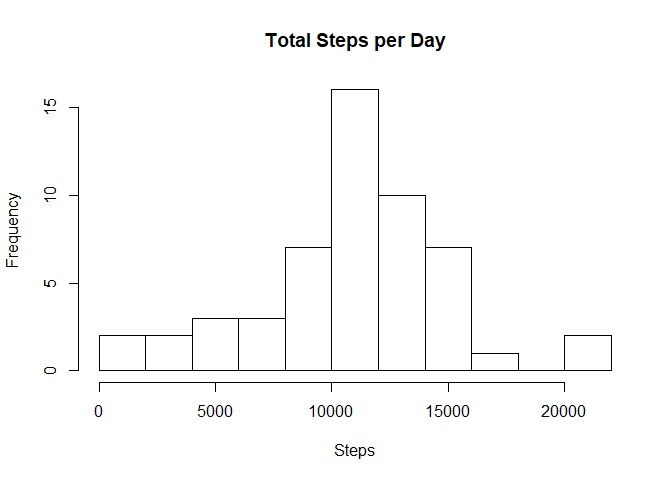
\includegraphics{PA1_template_files/figure-latex/unnamed-chunk-1-1.pdf}

\subsubsection{What are the mean and median total number of steps taken
per
day?}\label{what-are-the-mean-and-median-total-number-of-steps-taken-per-day}

\begin{Shaded}
\begin{Highlighting}[]
\NormalTok{movemean<-}\KeywordTok{as.integer}\NormalTok{(}\KeywordTok{mean}\NormalTok{(sumTable}\OperatorTok{$}\NormalTok{Steps))}
\NormalTok{movemedian<-}\KeywordTok{as.integer}\NormalTok{(}\KeywordTok{median}\NormalTok{(sumTable}\OperatorTok{$}\NormalTok{Steps))}
\end{Highlighting}
\end{Shaded}

The average total number of steps is 10766 and the median is 10765.

\subsubsection{What is the average daily activity
pattern?}\label{what-is-the-average-daily-activity-pattern}

\paragraph{Create average number of steps per
interval}\label{create-average-number-of-steps-per-interval}

\begin{Shaded}
\begin{Highlighting}[]
\NormalTok{intervalTable <-}\StringTok{ }\KeywordTok{ddply}\NormalTok{(clean, .(interval), summarize, }\DataTypeTok{Avg =} \KeywordTok{mean}\NormalTok{(steps))}
\end{Highlighting}
\end{Shaded}

\paragraph{Create line plot of average number of steps per
interval}\label{create-line-plot-of-average-number-of-steps-per-interval}

\begin{Shaded}
\begin{Highlighting}[]
\NormalTok{p <-}\StringTok{ }\KeywordTok{ggplot}\NormalTok{(intervalTable, }\KeywordTok{aes}\NormalTok{(}\DataTypeTok{x=}\NormalTok{interval, }\DataTypeTok{y=}\NormalTok{Avg), }\DataTypeTok{xlab =} \StringTok{"Interval"}\NormalTok{, }\DataTypeTok{ylab=}\StringTok{"Average Number of Steps"}\NormalTok{)}
\NormalTok{p }\OperatorTok{+}\StringTok{ }\KeywordTok{geom_line}\NormalTok{()}\OperatorTok{+}\KeywordTok{xlab}\NormalTok{(}\StringTok{"Interval"}\NormalTok{)}\OperatorTok{+}\KeywordTok{ylab}\NormalTok{(}\StringTok{"Average Number of Steps"}\NormalTok{)}\OperatorTok{+}\KeywordTok{ggtitle}\NormalTok{(}\StringTok{"Average Number of Steps per Interval"}\NormalTok{)}
\end{Highlighting}
\end{Shaded}

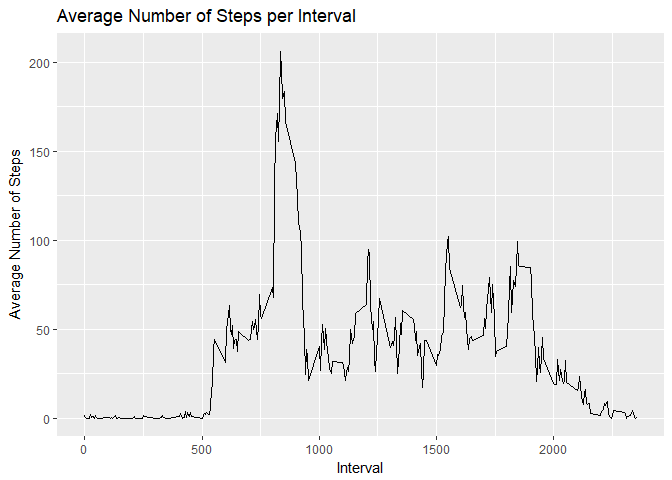
\includegraphics{PA1_template_files/figure-latex/unnamed-chunk-4-1.pdf}

\begin{Shaded}
\begin{Highlighting}[]
\NormalTok{##Maximum steps by interval}
\NormalTok{maxSteps <-}\StringTok{ }\KeywordTok{max}\NormalTok{(intervalTable}\OperatorTok{$}\NormalTok{Avg)}
\NormalTok{##Which interval contains the maximum average number of steps}
\NormalTok{intervalTable[intervalTable}\OperatorTok{$}\NormalTok{Avg}\OperatorTok{==}\NormalTok{maxSteps,}\DecValTok{1}\NormalTok{]}
\end{Highlighting}
\end{Shaded}

\begin{verbatim}
## [1] 835
\end{verbatim}

The maximum number of steps for a 5-minute interval was 206.1698113
steps.

The 5-minute interval which had the maximum number of steps was the 835
interval.

\paragraph{Imputing missing values}\label{imputing-missing-values}

Calculate and report the total number of missing values in the dataset
(i.e.~the total number of rows with NAs)

\begin{Shaded}
\begin{Highlighting}[]
\NormalTok{##Number of NAs in original data set}
\NormalTok{missing<-}\KeywordTok{nrow}\NormalTok{(movement[}\KeywordTok{is.na}\NormalTok{(movement}\OperatorTok{$}\NormalTok{steps),])}
\end{Highlighting}
\end{Shaded}

The number of rows with missing data is 2304. Impute the missing values
by substituting the missing steps with the average 5-minute interval
based on the day of the week. Then create a new dataset that is equal to
the original dataset but with the missing data filled in.

\begin{Shaded}
\begin{Highlighting}[]
\NormalTok{## Create the average number of steps per weekday and interval}
\NormalTok{avgTable <-}\StringTok{ }\KeywordTok{ddply}\NormalTok{(clean, .(interval, date), summarize, }\DataTypeTok{Avg =} \KeywordTok{mean}\NormalTok{(steps))}
\NormalTok{## Create dataset with all NAs for substitution}
\NormalTok{nadata<-}\StringTok{ }\NormalTok{movement[}\KeywordTok{is.na}\NormalTok{(movement}\OperatorTok{$}\NormalTok{steps),]}
\NormalTok{## Merge NA data with average weekday interval for substitution}
\NormalTok{newdata<-}\KeywordTok{merge}\NormalTok{(nadata, avgTable, }\DataTypeTok{by=}\KeywordTok{c}\NormalTok{(}\StringTok{"interval"}\NormalTok{, }\StringTok{"date"}\NormalTok{))}
\NormalTok{## Reorder the new substituded data in the same format as clean data set}
\NormalTok{newdata2<-}\StringTok{ }\NormalTok{newdata[,}\KeywordTok{c}\NormalTok{(}\DecValTok{6}\NormalTok{,}\DecValTok{4}\NormalTok{,}\DecValTok{1}\NormalTok{,}\DecValTok{2}\NormalTok{,}\DecValTok{5}\NormalTok{)]}
\KeywordTok{colnames}\NormalTok{(newdata2)<-}\StringTok{ }\KeywordTok{c}\NormalTok{(}\StringTok{"steps"}\NormalTok{, }\StringTok{"date"}\NormalTok{, }\StringTok{"interval"}\NormalTok{, }\StringTok{"day"}\NormalTok{, }\StringTok{"DateTime"}\NormalTok{)}
\NormalTok{##Merge the NA averages and non NA data together}
\NormalTok{mergeData <-}\StringTok{ }\KeywordTok{rbind}\NormalTok{(clean, newdata2)}
\end{Highlighting}
\end{Shaded}

Next, we make a histogram of the total number of steps taken each day
and Calculate and report the mean and median total number of steps taken
per day.

\begin{Shaded}
\begin{Highlighting}[]
\NormalTok{##Create sum of steps per date to compare with step 1}
\NormalTok{sumTable2 <-}\StringTok{ }\KeywordTok{aggregate}\NormalTok{(mergeData}\OperatorTok{$}\NormalTok{steps }\OperatorTok{~}\StringTok{ }\NormalTok{mergeData}\OperatorTok{$}\NormalTok{date, }\DataTypeTok{FUN=}\NormalTok{sum, )}
\KeywordTok{colnames}\NormalTok{(sumTable2)<-}\StringTok{ }\KeywordTok{c}\NormalTok{(}\StringTok{"Date"}\NormalTok{, }\StringTok{"Steps"}\NormalTok{)}
\NormalTok{## Mean of Steps with NA data taken care of}
\NormalTok{imputedMean<-}\KeywordTok{as.integer}\NormalTok{(}\KeywordTok{mean}\NormalTok{(sumTable2}\OperatorTok{$}\NormalTok{Steps))}
\NormalTok{## Median of Steps with NA data taken care of}
\NormalTok{imputedMedian<-}\KeywordTok{as.integer}\NormalTok{(}\KeywordTok{median}\NormalTok{(sumTable2}\OperatorTok{$}\NormalTok{Steps))}
\end{Highlighting}
\end{Shaded}

The average total number of steps is 10766 and the median is 10765.

\begin{Shaded}
\begin{Highlighting}[]
\NormalTok{## Creating the histogram of total steps per day, categorized by data set to show impact}
\KeywordTok{hist}\NormalTok{(sumTable2}\OperatorTok{$}\NormalTok{Steps, }\DataTypeTok{breaks=}\DecValTok{10}\NormalTok{, }\DataTypeTok{xlab=}\StringTok{"Steps"}\NormalTok{, }\DataTypeTok{main =} \StringTok{"Total Steps per Day with NAs Fixed"}\NormalTok{, }\DataTypeTok{col=}\StringTok{"Black"}\NormalTok{)}
\KeywordTok{hist}\NormalTok{(sumTable}\OperatorTok{$}\NormalTok{Steps, }\DataTypeTok{breaks=}\DecValTok{10}\NormalTok{, }\DataTypeTok{xlab=}\StringTok{"Steps"}\NormalTok{, }\DataTypeTok{main =} \StringTok{"Total Steps per Day with NAs Fixed"}\NormalTok{, }\DataTypeTok{col=}\StringTok{"White"}\NormalTok{, }\DataTypeTok{add=}\NormalTok{T)}
\KeywordTok{legend}\NormalTok{(}\StringTok{"topright"}\NormalTok{, }\KeywordTok{c}\NormalTok{(}\StringTok{"Imputed Data"}\NormalTok{, }\StringTok{"Non-NA Data"}\NormalTok{), }\DataTypeTok{fill=}\KeywordTok{c}\NormalTok{(}\StringTok{"black"}\NormalTok{, }\StringTok{"white"}\NormalTok{) )}
\end{Highlighting}
\end{Shaded}

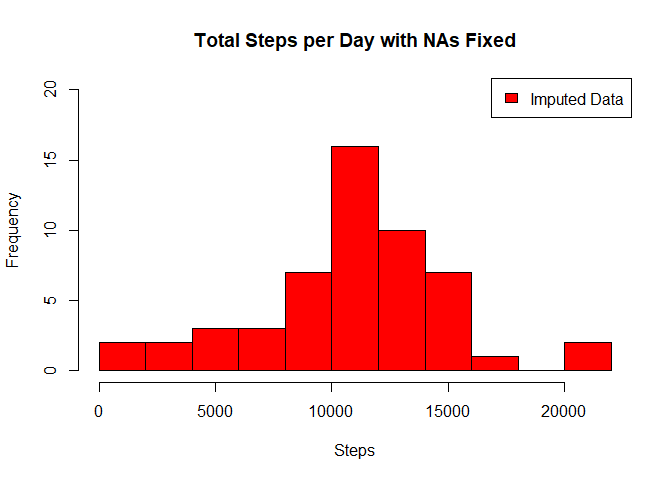
\includegraphics{PA1_template_files/figure-latex/unnamed-chunk-9-1.pdf}

\subsubsection{Are there differences in activity patterns between
weekdays and
weekends?}\label{are-there-differences-in-activity-patterns-between-weekdays-and-weekends}


\end{document}
